\chapter{Design Calculations}
\label{ch:design_calculations}

This appendix presents the quantitative structural and electromagnetic sizing calculations for the PCMA joint mechanism.

\section{Articulating Link Mass and Holding Torque Verification}
\label{sec:link_mass_calc}

To verify whether TPM\_03 remains valid for the finalized joint geometry, the mass of the articulating link assembly, comprising the aluminium link pipe, probe hub, and steel measuring probe, was calculated, under Equation~\ref{eq:Articulation_link_weight_app} below. An aluminium density of $\rho_{\text{Al}} = \SI{2700}{kg/m^3}$ and a steel density of $\rho_{\text{steel}} = \SI{7850}{kg/m^3}$ was assumed, using the FBD and safety factor ($\text{SF} = 1.5$) established under Section~3.4.3 \citep{Hibbler:2017}.

\begin{equation}
	\label{eq:Articulation_link_weight_app}
	\begin{aligned}
		m_{\text{link}} &= \rho_{\text{Al}} \cdot V_{\text{pipe}} + \rho_{\text{Al}} \cdot V_{\text{hub}} + \rho_{\text{steel}} \cdot V_{\text{probe}} \\
		&= \rho_{\text{Al}} \left[ \pi (r_o^2 - r_i^2) L_{\text{pipe}} + \pi (r_{\text{top}}^2 + r_{\text{bottom}}^2) L_{\text{hub}} \right] + \rho_{\text{steel}} \left[ \pi r_{\text{probe}}^2 L_{\text{probe}} \right] \\
		&= 2700 \cdot \Big[ \pi(0.016^2 - 0.013^2)(0.55) + \pi(0.017^2 + 0.013^2)(0.01) \Big] \\
		&\quad + 7850 \cdot \Big[ \pi(0.005^2)(0.1) \Big] \\
		&= \SI{0.4659}{kg} \\
		\therefore T_{\text{holding, verified}} &= \text{SF} \cdot m_{\text{link}} \cdot g \cdot l_{\text{link}} \\
		&= (1.5)(0.4659\,\mathrm{kg})(9.81\,\mathrm{m/s^2})(0.325\,\mathrm{m}) \\
		&= \SI{2.228}{N\cdot m}
	\end{aligned}
\end{equation}

Although Equation~\ref{eq:Articulation_link_weight_app} confirms that the physical link mass results in a required holding torque of \SI{2.228}{N.m}, the joint brake was conservatively sized against the upper-bound specification requirement of $T_{\text{holding}} = \SI{7.725}{N.m}$.

\section{Electromagnetic Brake Sizing and Axial Clamping Force}
\label{sec:brake_sizing_calc}

An outer diameter of $d_o = \SI{0.1}{m}$ and inner bore diameter of $d_i = \SI{0.022}{m}$ were chosen for the brake disc and friction plate interface based on the material available in the workshop and mechatronics laboratory, namely the mild steel piping and bars. 

Assuming uniform contact pressure across the rigid wood-on-steel friction interface ($\mu = 0.35$), the required axial clamping force $F_{\text{clamping}}$ to hold $T_{\text{holding}} = \SI{7.725}{N.m}$ is derived from Shigley's uniform pressure disk brake model \citep{Shigley:2015}:

\begin{equation}
	\label{eq:F_holding_app}
	\begin{aligned}
		T_{\text{holding}} &= \frac{2}{3} \mu F_{\text{clamping}} \left( \frac{r_o^3 - r_i^3}{r_o^2 - r_i^2} \right) \\[1ex]
		\Rightarrow F_{\text{clamping}} &= \frac{3 \cdot T_{\text{holding}}}{2 \cdot \mu }\left( \frac{r_o^3 - r_i^3}{r_o^2 - r_i^2} \right) \\
		&= \frac{3 \cdot (7.725)}{2 \cdot (0.35) } \left( \frac{0.050^2 - 0.011^2}{0.050^3 - 0.011^3} \right)\\
		&= \SI{636.88}{N}
	\end{aligned}
\end{equation}

\section{Circuit Sizing and Electromagnet Winding Derivations}
\label{app:design_calc}

\subsection{Component Voltage, Current, and Power Distribution}
Table~\ref{tab:circuit_operating_params} details the operating parameters (obtained from the component's respective datasheets) across each node during active steady-state operation at $I_{\text{total}} = 8\text{ A}$.

\begin{table}[h]
	\centering
	\caption{Electrical Operating Parameters Across Subsystem Nodes}
	\label{tab:circuit_operating_params}
	\resizebox{\linewidth}{!}{%
		\begin{tabular}{lccc}
			\hline
			\textbf{Subsystem / Component} & \textbf{Node Voltage ($V$)} & \textbf{Operating Current} & \textbf{Power ($W$)} \\ \hline
			STM32 GPIO Signal               & $3.3\text{ V}_{\text{DC}}$    & $2.6\text{ mA}$            & $8.6\text{ mW}$      \\
			2N3904 Pre-Driver Base         & $0.7\text{ V}_{\text{BE}}$    & $2.6\text{ mA}$            & $1.8\text{ mW}$      \\
			2N3904 Collector ($V_{CE}$)    & $0.2\text{ V}_{\text{sat}}$   & $5.4\text{ mA}$            & $1.1\text{ mW}$      \\
			IRF640N Gate ($V_{GS}$)        & $12.0\text{ V}_{\text{DC}}$   & $< 1\text{ mA}$            & $< 10\text{ mW}$     \\
			Solenoids (4$\times$ Parallel)  & $24.0\text{ V}_{\text{DC}}$   & $8.0\text{ A}$ (total)     & $192.0\text{ W}$     \\
			XL7015 DC-DC Converter         & $24.0\text{ V}_{\text{DC}}$   & $0.12\text{ A}$            & $2.88\text{ W}$      \\
			GTS06 Optical Encoder          & $5.0\text{ V}_{\text{DC}}$    & $60\text{ mA}$             & $0.30\text{ W}$      \\
			IRF640N MOSFET Drain-Source    & $1.2\text{ V}_{\text{drop}}$  & $8.0\text{ A}$             & $9.60\text{ W}$      \\ \hline
		\end{tabular}%
	}
\end{table}

\subsection{Electromagnet Winding Design based on Clamping Force}
To determine the required turn count ($N$) per solenoid, the total magnetic force ($F_{\text{mag}}$) generated by the electromagnet is equated directly to the required normal clamping force ($F_{\text{clamping}}$) of the brake.

\subsubsection{Air Gap Magnetic Flux Density ($B$)}
The magnetic force exerted across the effective cross-sectional area of the electromagnetic brake $A_e = \pi(0.1)^2 = \SI{31.42e-3}{m^2}$ with a working air gap $g = 0.3\text{ mm} = 3 \times 10^{-4}\text{ m}$ is expressed by Maxwell's stress tensor from Equation~\ref{eq:24rwkg} under Section 2.4.2.

Solving for the required magnetic flux density $B$, under Equation~\ref{eq:kvbf}:
\begin{equation}
	\label{eq:kvbf}
	B = \sqrt{\frac{2 \mu_0 \cdot \mathcal{F}}{A_e}} = \sqrt{\frac{2 \cdot (4\pi \times 10^{-7}\text{ H/m}) \cdot 636.88\text{ N}}{31.42 \times 10^{-3}\text{ m}^2}} \approx 0.2257\text{ T}
\end{equation}

\subsubsection{Turn Sizing ($N$) per Solenoid}
Neglecting iron core reluctance ($\mu_{\text{core}} \gg \mu_0$), the total Magnetomotive Force (MMF) required across the air gap $g$ for a parallel circuit setup is stated under Equation~\ref{eq:24rwkg} under Section 2.4.2, where $\mathcal{F}=F_{\text{clamping}}$.

Therefore, solving for the minimum required turns per solenoid, as seen in Equation~\ref{eq:jvzljnb}:
\begin{equation}
	\label{eq:jvzljnb}
	N_{\text{solenoid}} = \sqrt{\frac{\mathcal{F}(2g^2)}{kI_{\text{total}^2}\mu_0A_g}} = \sqrt{\frac{636.88[2(3\times10^{-3})^2]}{4(8)^2(4\pi \times10^{-7})(\pi(0.015)^2)}}\approx \SI{225}{\text{coils per solenoid}}
\end{equation}

Applying a $15\%$ safety factor to compensate for magnetic flux leakage and core reluctance losses:
\begin{equation}
	N_{\text{design}} = \lceil 225 \times 1.15 \rceil = 259\text{ turns per solenoid}
\end{equation}

\section{Electromagnet Actuation Force and Winding Derivations}
\label{app:winding_calc}

\subsection{Mechanical Actuation Force Threshold ($F_{e(\text{new})}$)}
Physical actuation of the electromagnetic brake requires deflecting the mild steel pressure tabs by $g = \SI{3}{mm} = \SI{0.003}{m}$. Modeling each pressure tab as a cantilever beam, the required tip deflection force is:
\begin{equation}
	F_{e(\text{new})} = \frac{3 g E I}{L^3}
\end{equation}

Given Young's modulus $E = \SI{210}{GPa}$, length $L = \SI{0.029077}{m}$, width $b = \SI{0.020}{m}$, and thickness $t = \SI{0.001}{m}$, the second moment of area $I$ is calculated as:
\begin{equation}
	I = \frac{1}{12} b t^3 = \frac{1}{12} (0.020\text{ m})(0.001\text{ m})^3 = 1.667 \times 10^{-12}\text{ m}^4
\end{equation}

Substituting these parameters yields the revised minimum actuation force threshold:
\begin{equation}
	F_{e(\text{new})} = \frac{3(0.003\text{ m})(210 \times 10^9\text{ Pa})(1.667 \times 10^{-12}\text{ m}^4)}{(0.029077\text{ m})^3} \approx \SI{128.1}{N}
\end{equation}

Dividing across $N_{\text{sol}} = 4$ solenoids gives the minimum required force per individual coil:
\begin{equation}
	F_{\text{sol}} = \frac{F_{e(\text{new})}}{4} = \frac{128.1\text{ N}}{4} \approx \SI{32.03}{N}
\end{equation}

\subsection{Air Gap Flux Density ($B$) and Required Magnetomotive Force ($\mathcal{F}$)}
Using Maxwell's stress tensor, the magnetic flux density $B$ required to generate $F_{\text{sol}} = \SI{32.03}{N}$ across an effective pole area $A_p = 1.8 \times 10^{-4}\text{ m}^2$ is:
\begin{equation}
	B = \sqrt{\frac{2 \mu_0 F_{\text{sol}}}{A_p}} = \sqrt{\frac{2 (4\pi \times 10^{-7}\text{ H/m})(32.03\text{ N})}{1.8 \times 10^{-4}\text{ m}^2}} \approx \SI{0.669}{T}
\end{equation}

Neglecting iron core reluctance ($\mu_{\text{core}} \gg \mu_0$), the Magnetomotive Force ($\mathcal{F}$) required across an air gap $g = \SI{0.5}{mm} = 5 \times 10^{-4}\text{ m}$ is:
\begin{equation}
	\mathcal{F} = N \cdot I_{\text{sol}} = \frac{B \cdot g}{\mu_0} = \frac{(0.669\text{ T})(5 \times 10^{-4}\text{ m})}{4\pi \times 10^{-7}\text{ H/m}} \approx 266.2\text{ A}\cdot\text{turns}
\end{equation}

\subsection{Theoretical vs. As-Built Turn Sizing Comparison}

The equivalent resistance and inductance parameters of the individual solenoids and the total electromagnet were derived to configure the LTspice simulation. The static DC resistance of a single solenoid is determined by Equation~\ref{eq:R_sol1}:
\begin{equation}
	\label{eq:R_sol1}
	R_{\text{sol}} = \rho \frac{l_w}{A_w}
\end{equation}
where $\rho = \SI{17.02}{n\Omega/m}$ is the electrical resistivity of copper at room temperature, $l_w$ is the total length of wire, and $A_w$ is the cross-sectional area of the wire conductor. The self-inductance of a single solenoid is determined by Equation~\ref{eq:L_sol1}:
\begin{equation}
	\label{eq:L_sol1}
	L_{\text{sol}} = \frac{\mu N_{\text{solenoid}}^2 A_c}{l_c}
\end{equation}
where $\mu = \mu_0 \mu_r$ is the magnetic permeability of the mild steel solenoid core (assuming $\mu_r \approx 2000$ for the steel core), $A_c$ is the cross-sectional area of the core, and $l_c$ is the magnetic path length. For calculation purposes, the conductor length $l_w$ and magnetic path length $l_c$ were assumed equal.

The theoretical resistance and inductance values for a single solenoid, as well as the equivalent values for the four-solenoid parallel array, are derived in Equation~\ref{eq:R_sol1_and_L_sol1}:
\begin{align}
	\label{eq:R_sol1_and_L_sol1}
	R_{\text{sol}} &= (17.02 \times 10^{-9})\frac{2\pi(0.015)\left[\frac{2(100)}{0.28}\right]}{\pi(140 \times 10^{-6})^2} \approx \SI{18.61}{\Omega} \\
	\mu &= \mu_0 \mu_r = (4\pi \times 10^{-7})(2000) \approx \SI{2.513e-3}{H/m} \\
	L_{\text{sol}} &= \frac{(2.513 \times 10^{-3})(715)^2 \left[\pi (0.015)^2\right]}{2\pi(0.015)\left[\frac{2(100)}{0.28}\right]} \approx \SI{13.49}{mH} \\
	R_{\text{eq,calc}} &= \frac{R_{\text{sol}}}{4} = \frac{\SI{18.61}{\Omega}}{4} = \SI{4.65}{\Omega} \\
	L_{\text{eq,calc}} &= \frac{L_{\text{sol}}}{4} = \frac{\SI{13.49}{mH}}{4} \approx \SI{3.37}{mH}
\end{align}

\section{LTspice Circuit Simulations and Experimental Validation}
\label{app:circuit_simulations}

To verify the switching response, component stress limits, and signal amplification of the switching circuit before to hardware implementation, transient analysis simulations were executed in LTspice, as seen by Figure~\ref{fig:LTSpice_SIM}.
\begin{figure}[H]
	\centering
	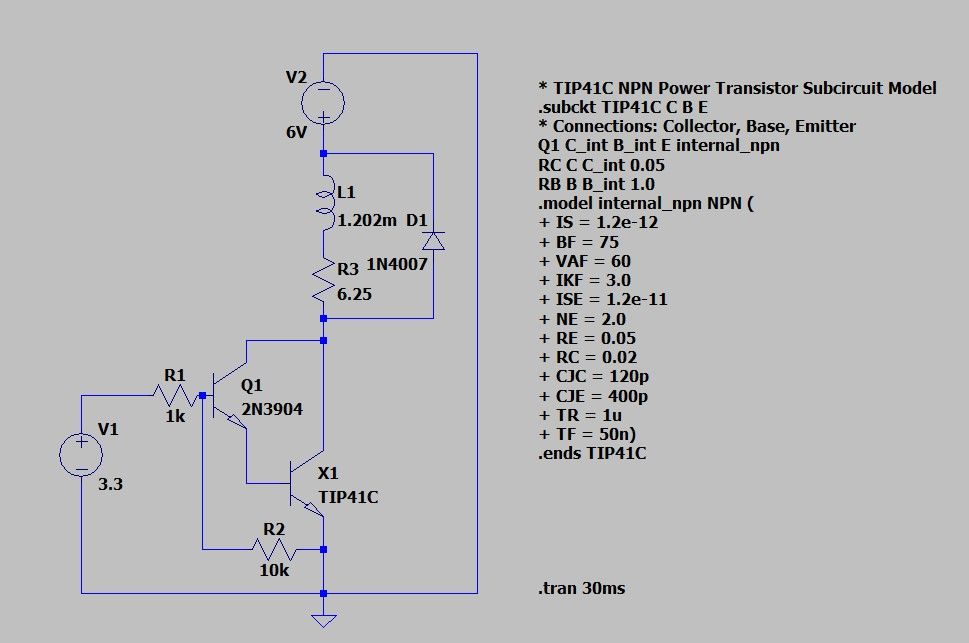
\includegraphics[width=0.7\linewidth]{LTspice model of Switching Circuit.jpg}
	\caption{LTSpice Model}
	\label{fig:LTSpice_SIM}
\end{figure}

\subsection{Switching Circuit Component Sizing Derivations}
\label{app:switching_calc}

To drive the electromagnetic load from a \SI{3.3}{V} STM32 GPIO signal without exceeding pin current thresholds, a low-side Darlington driver stage pairing a 2N3904 BJT with a TIP41C power transistor was sized.

\subsubsection{TIP41C Forced Saturation Sizing}
To maintain low collector-emitter saturation voltage ($V_{CE(\text{sat})} \le \SI{1.0}{V}$) at a maximum load current of $I_C = \SI{831.75}{mA}$, a forced saturation gain of $\beta_2 = 15$ was enforced. The required base drive current $I_{B2}$ for the TIP41C is:
\begin{equation}
	I_{B2} = \frac{I_C}{\beta_2} = \frac{\SI{831.75}{mA}}{15} = \SI{55.45}{mA}
\end{equation}

\subsubsection{2N3904 and Base Resistor ($R_B$) Sizing}
The 2N3904 amplifies the GPIO input current to deliver $I_{C1} = I_{B2} = \SI{55.45}{mA}$. Applying a forced gain of $\beta_1 = 20$ for the 2N3904 yields the required GPIO input current:
\begin{equation}
	I_{B1} = \frac{I_{C1}}{\beta_1} = \frac{\SI{55.45}{mA}}{20} \approx \SI{2.77}{mA}
\end{equation}

The base current-limiting resistor $R_B$ is calculated using Kirchhoff's Voltage Law across the \SI{3.3}{V} logic signal ($V_{\text{GPIO}}$) and base-emitter drop ($V_{BE1} = \SI{0.70}{V}$):
\begin{equation}
	R_B = \frac{V_{\text{GPIO}} - V_{BE1}}{I_{B1}} = \frac{\SI{3.3}{V} - \SI{0.70}{V}}{\SI{2.77}{mA}} \approx \SI{938.6}{\Omega}
\end{equation}
Selecting a standard nominal resistor of $R_B = \SI{1.0}{k\Omega}$ limits the microcontroller pin current to a safe value of $I_{\text{GPIO}} = \SI{2.60}{mA}$.

\subsubsection{Transistor Power Dissipation ($P_D$)}
Total continuous power dissipation in the TIP41C during active conduction is calculated as:
\begin{equation}
	\begin{aligned}
		P_{\text{D(TIP41C)}} &= (V_{CE(\text{sat})} \cdot I_C) + (V_{BE2} \cdot I_{B2}) \\
		&= (0.801\text{ V})(0.832\text{ A}) + (1.10\text{ V})(0.055\text{ A}) \approx \SI{0.727}{W}
	\end{aligned}
\end{equation}
This confirms that continuous thermal dissipation stays well within safe limits when fitted with standard TO-220 aluminum heatsinks.

\subsection{Signal Amplification and Collector Current Response}
Figure~\ref{fig:signal-amplification-from-input-to-electromagnet} illustrates the current amplification from the microcontroller GPIO signal input (modelled as the V1 voltage supply) to the electromagnet load. The input signal current $I(V1)$ remains below \SI{1}{mA}, while the switching transistor delivers a steady load current of $I(R3) = \SI{831.75}{mA}$ through the solenoid array.

\begin{figure}[H]
	\centering
	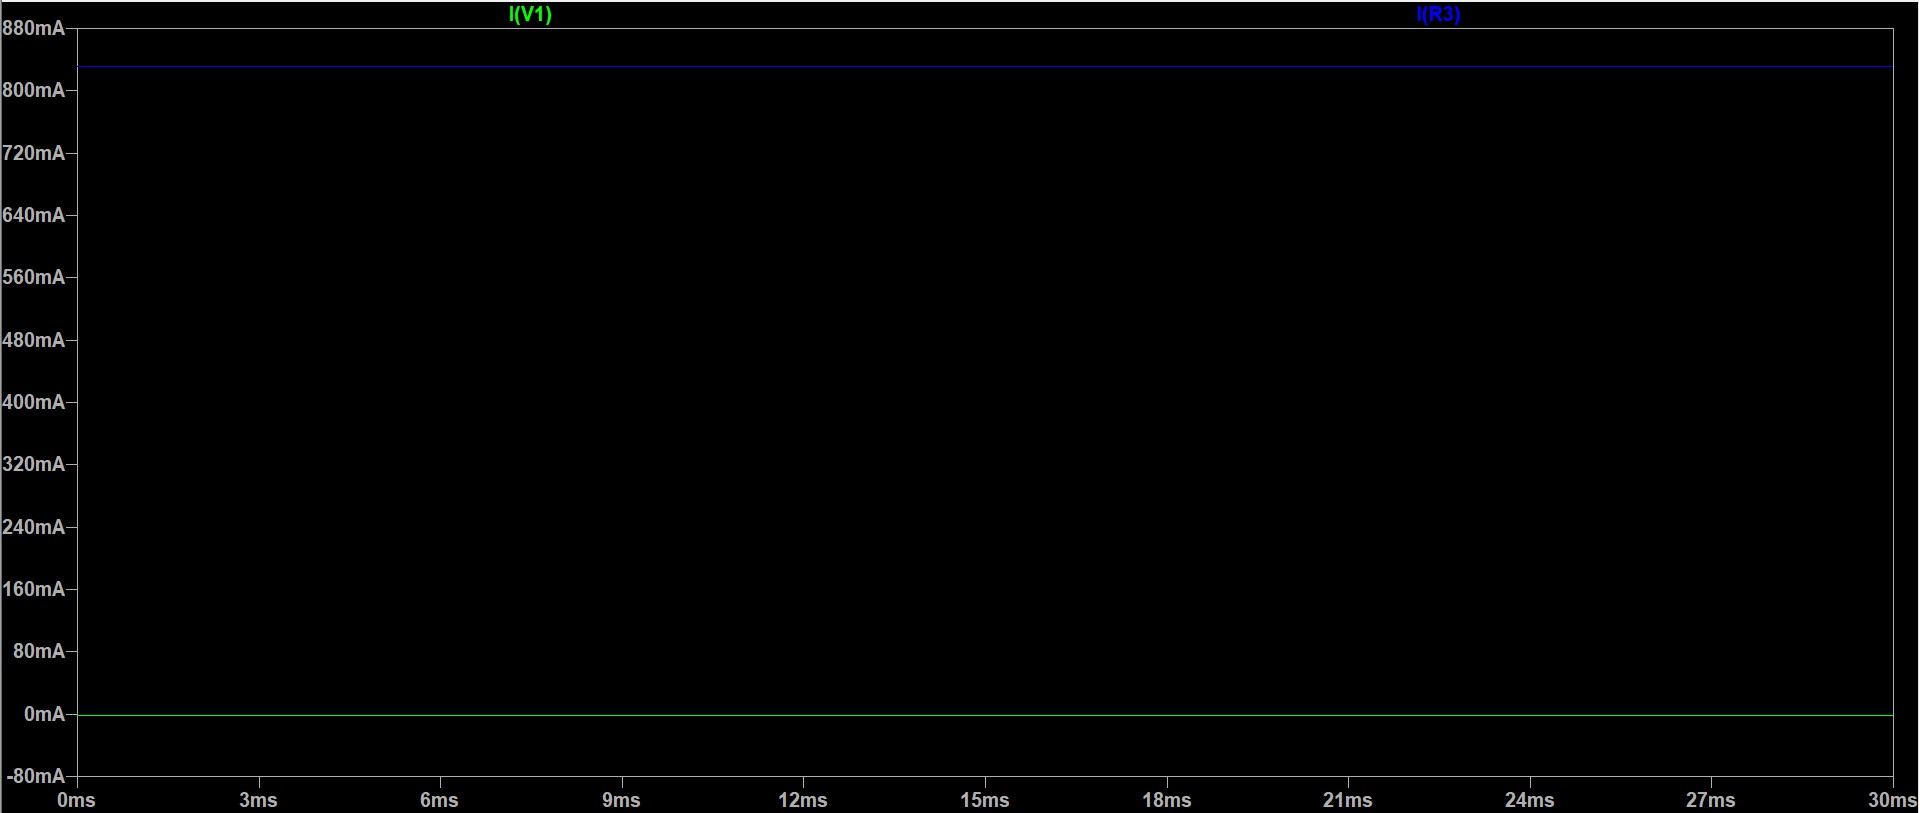
\includegraphics[width=0.9\linewidth]{Signal amplification from input to electromagnet.jpg}
	\caption{LTspice Simulation: Input GPIO Signal Current $I(V1)$ vs. Amplified Solenoid Load Current $I(R3) = \SI{831.75}{mA}$}
	\label{fig:signal-amplification-from-input-to-electromagnet}
\end{figure}

\subsection{Inductive Switching Response and Coil Current Decay}
Figure~\ref{fig:electromagnetic-inductance} demonstrates the transient current behavior $I(L1)$ across the electromagnet coil inductance. Upon turn-off, the freewheeling 1N4007 flyback diode provides a safe recirculation path for the collapsing magnetic field energy, clamping inductive Back-EMF spikes and protecting the TIP41C collector-emitter junction.
\begin{figure}[H]
	\centering
	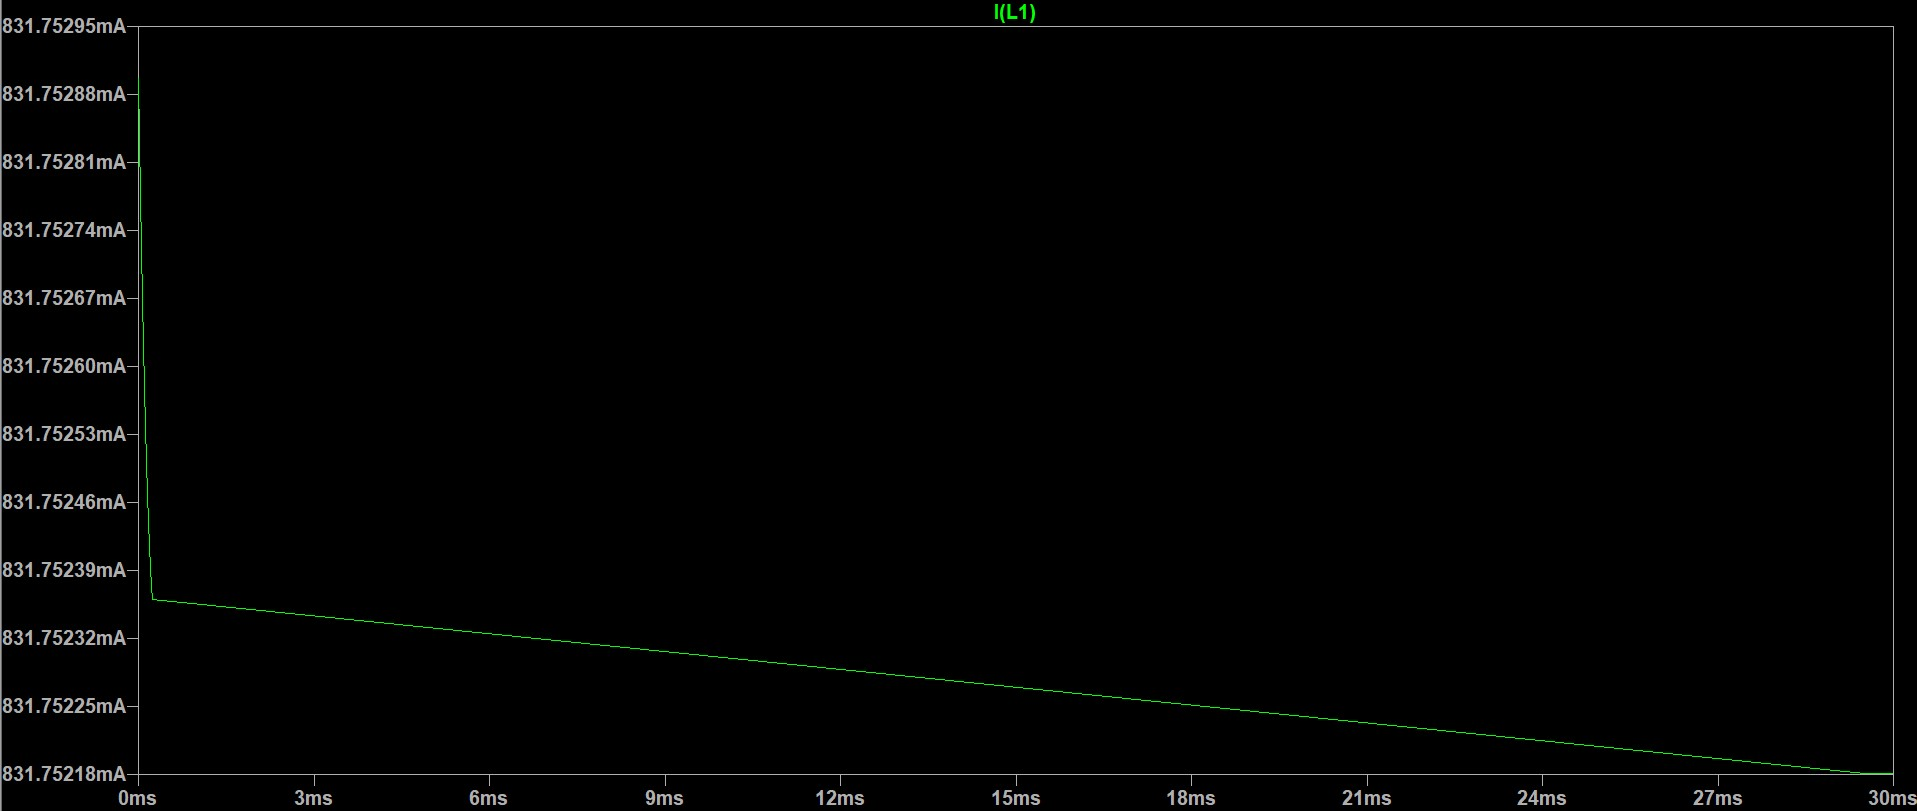
\includegraphics[width=0.9\linewidth]{Electromagnetic Inductance.jpg}
	\caption{LTspice Simulation: Inductive Coil Current Transient $I(L1)$ During Switching Operations}
	\label{fig:electromagnetic-inductance}
\end{figure}

\subsection{Transistor Collector-Emitter Saturation Voltage ($V_{CE}$)}
Figure~\ref{fig:vce-across-tip41c-transistor-and-ic-from-electromagnet} details the collector-emitter voltage $V(n003)$ and collector current $I(R3)$ across the TIP41C power transistor. At a cursor timestamp of $t = \SI{26.56}{ms}$, the simulation confirms full saturation with $V_{CE} = \SI{800.72}{mV}$ (\SI{0.801}{V}) at $I_C = \SI{831.75}{mA}$. This aligns closely with the physical benchtop multimeter measurement of $V_{CE(\text{sat})} = \SI{0.95}{V}$ recorded in Figure~\ref{fig:20261013114913}.
\begin{figure}[H]
	\centering
	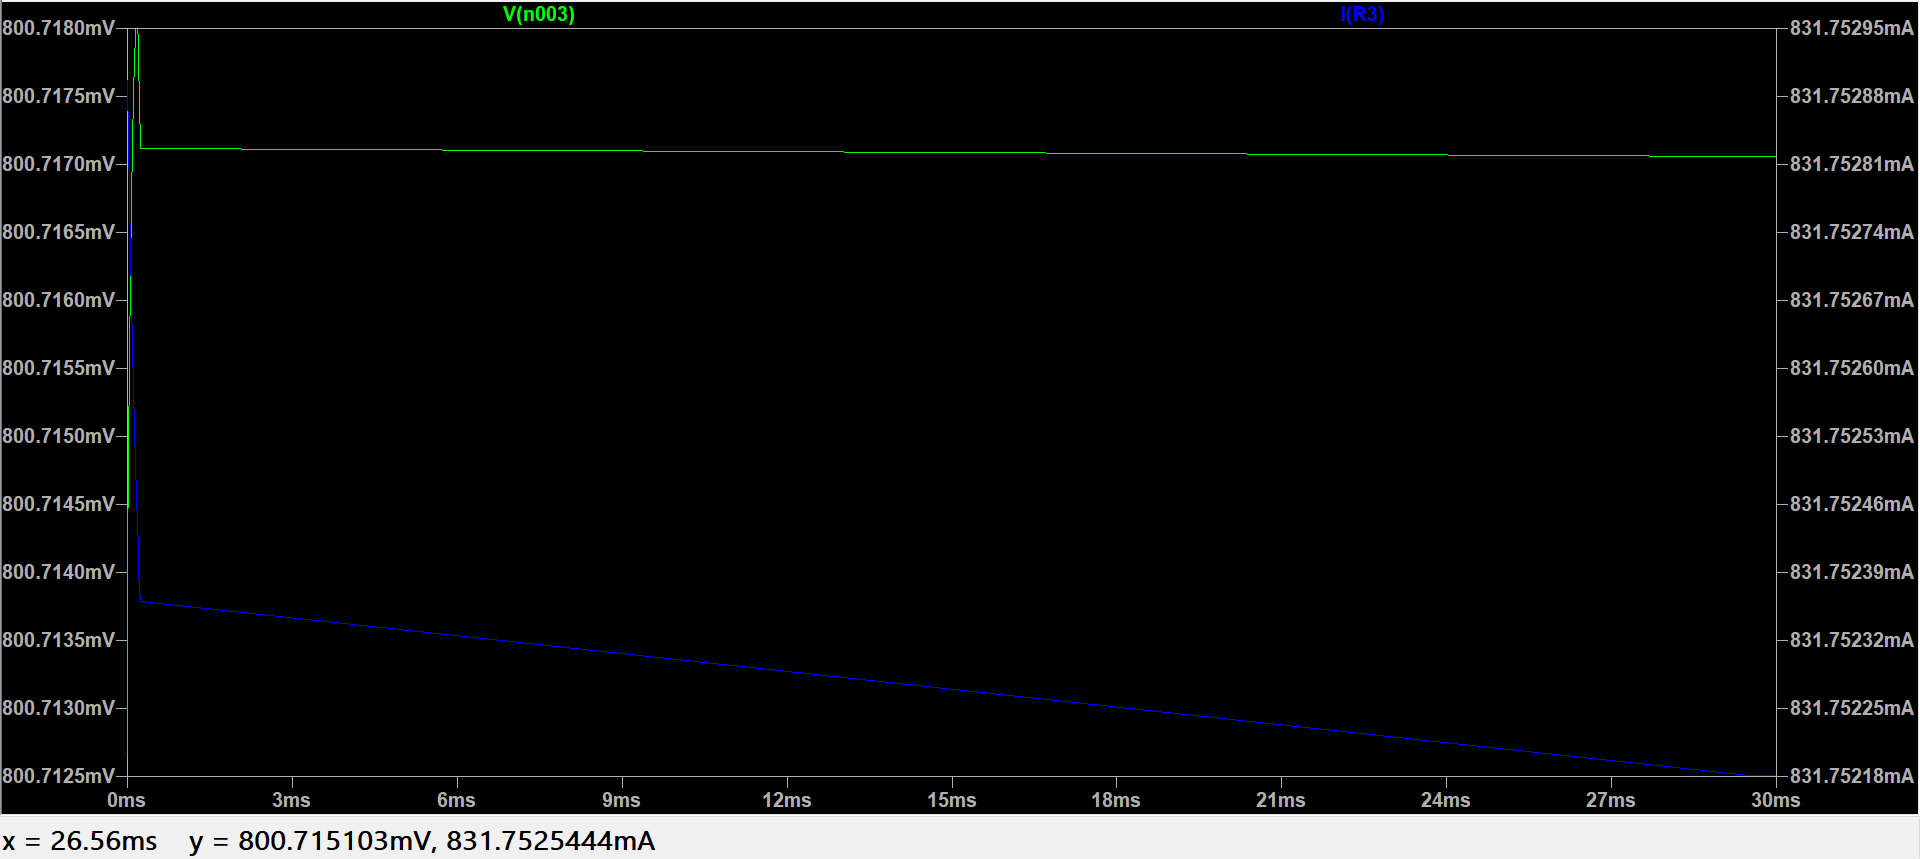
\includegraphics[width=0.9\linewidth]{Vce across TIP41C transistor and IC from electromagnet.png}
	\caption{LTspice Simulation: TIP41C Saturation Voltage $V_{CE} = \SI{800.72}{mV}$ and Collector Current $I_C = \SI{831.75}{mA}$ at $t = \SI{26.56}{ms}$}
	\label{fig:vce-across-tip41c-transistor-and-ic-from-electromagnet}
\end{figure}

\subsection{Power Dissipation in TIP41C Power Transistor}
Figure~\ref{fig:power-dissipation-in-tip41c} evaluates total instant power dissipation across the TIP41C transistor, calculated as $P_D = V_{CE} \cdot I_C + V_{BE} \cdot I_B$. The continuous power dissipation settles at $P_{\text{D(TIP41C)}} \approx \SI{666.82}{mW}$ (\SI{0.667}{W}) during steady-state conduction. This verifies that operating the driver continuously at nominal current will not exceed the package thermal threshold when fitted with standard TO-220 aluminum heatsinks.

\begin{figure}[H]
	\centering
	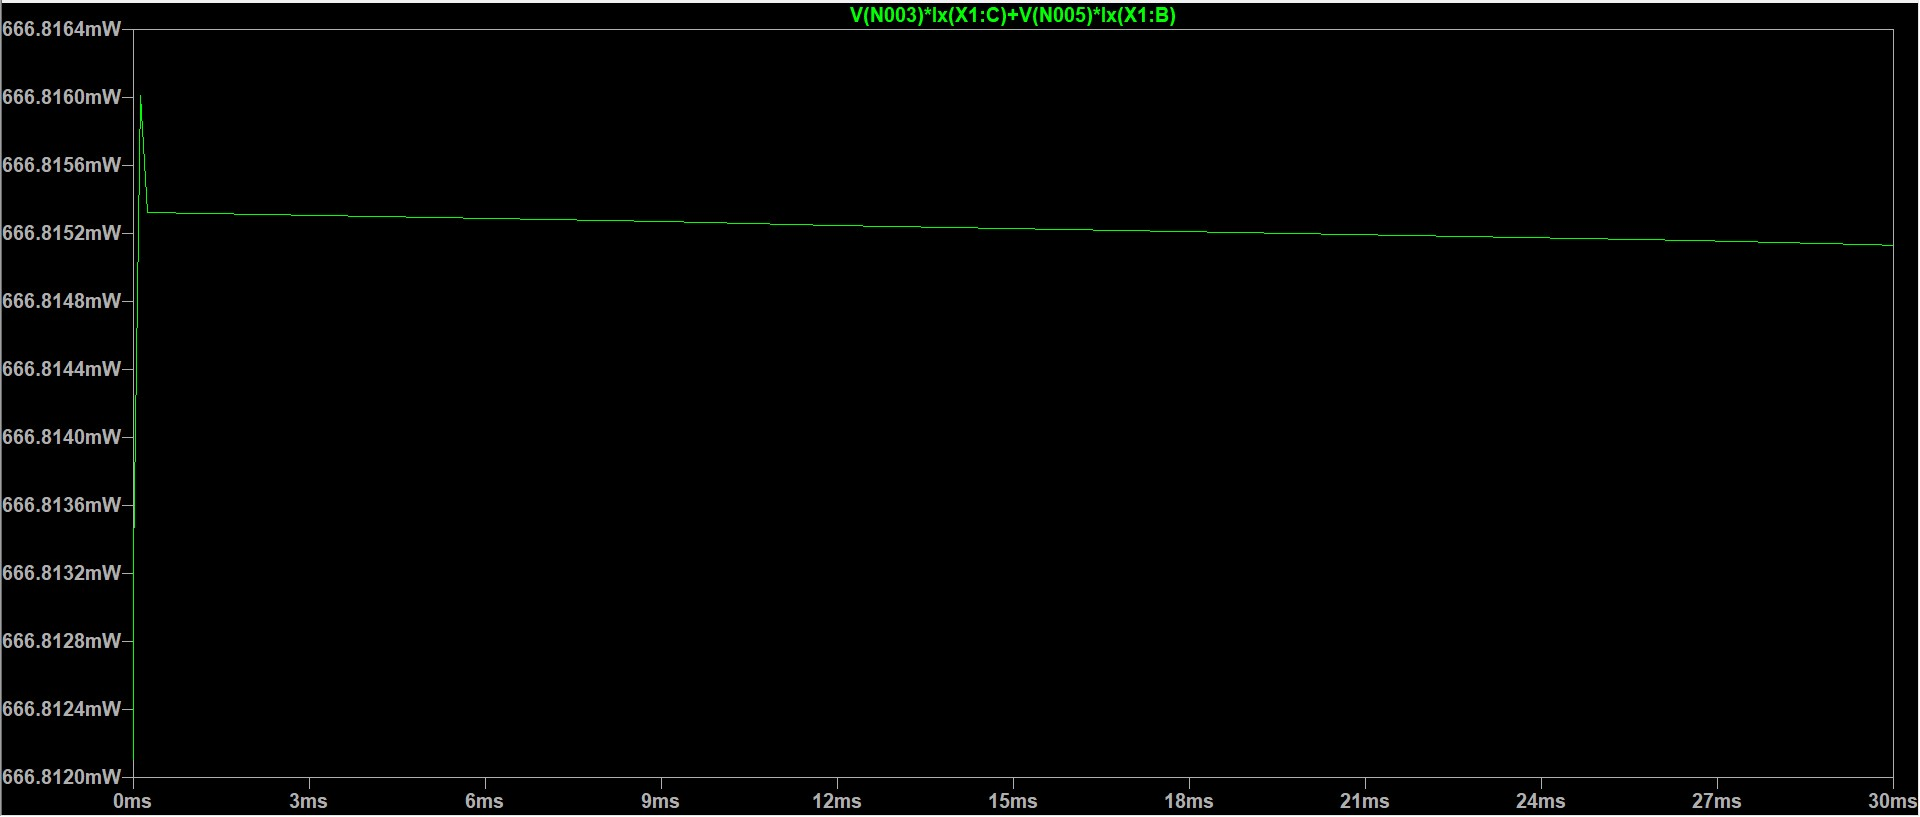
\includegraphics[width=0.9\linewidth]{Power dissipation in TIP41C.jpg}
	\caption{LTspice Simulation: Active Power Dissipation Trace across TIP41C Transistor ($P_D \approx \SI{666.82}{mW}$)}
	\label{fig:power-dissipation-in-tip41c}
\end{figure}

